\section{Ergebnis des zweiten Ideationszyklus mit der Lotus-Blossom-Methode} \label{appendix:lotus_blossom}

\begin{figure}[H]
  \centering
  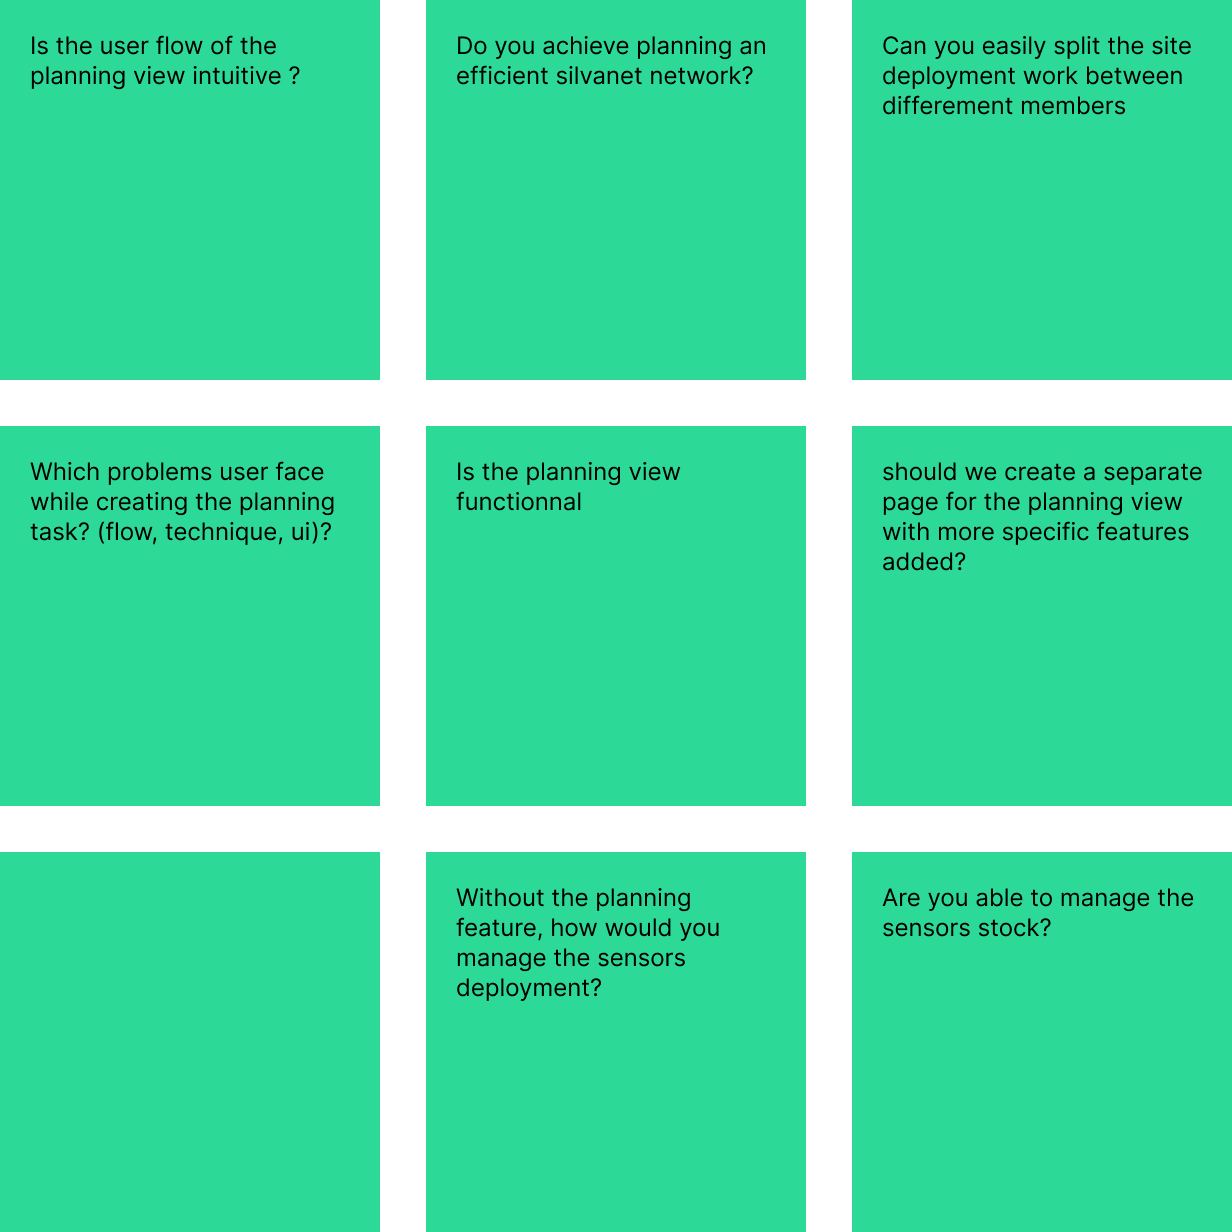
\includegraphics[width=10cm]{lotus_blossom_top}
  \caption{Ergebnis lotus blossom top}
  \label{fig:lotus_blossom_top}
\end{figure}
\begin{figure}[H]
  \centering
  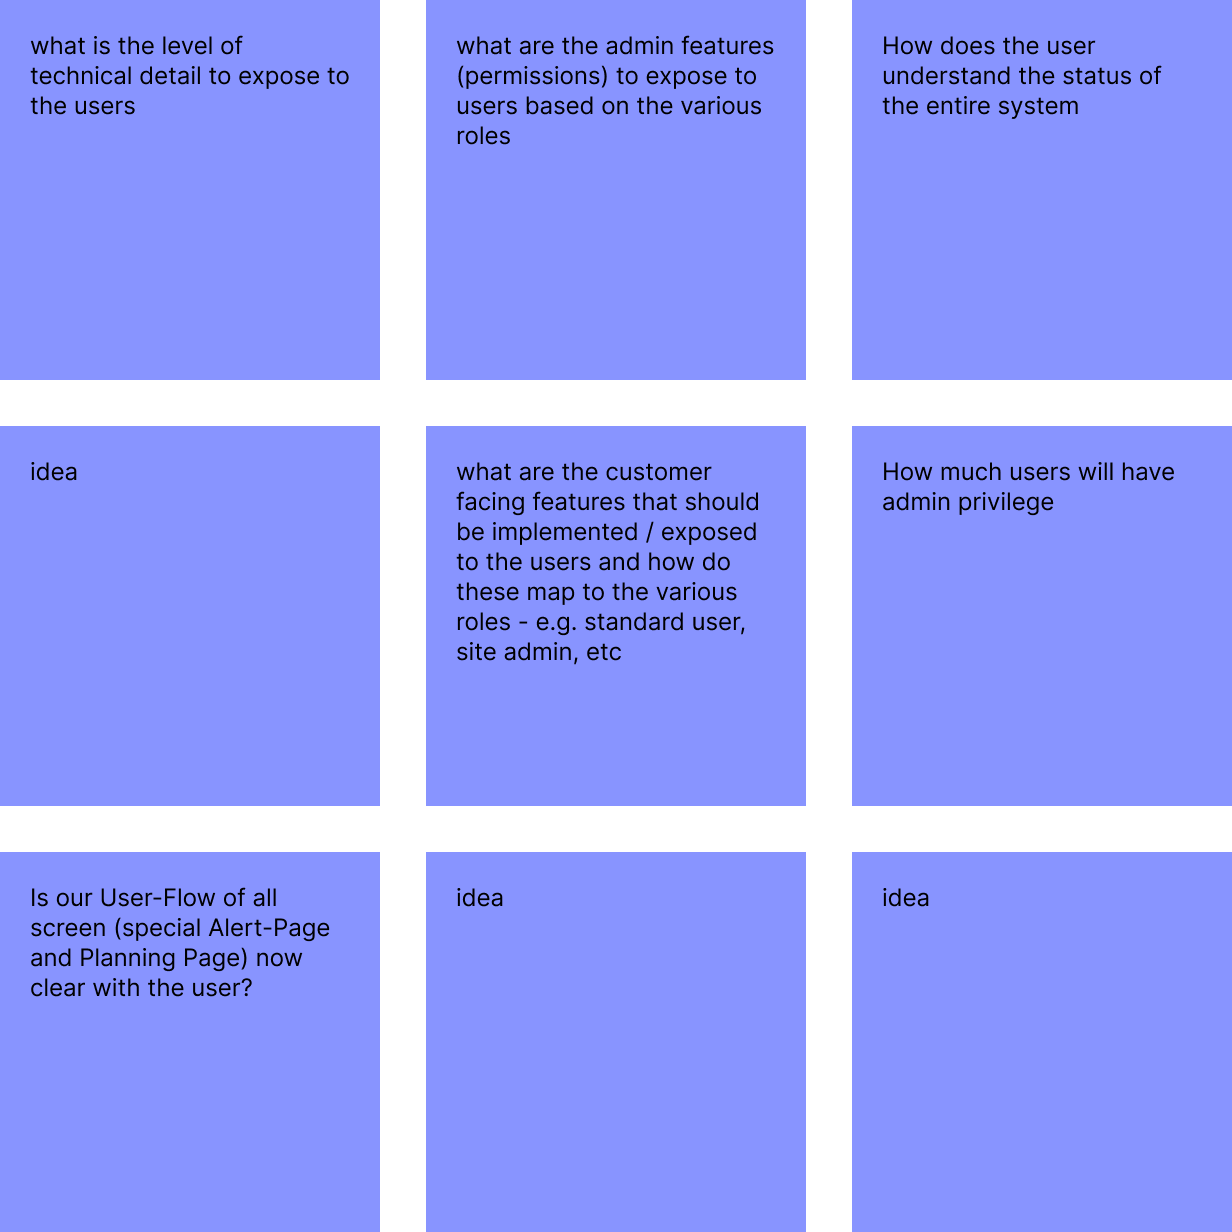
\includegraphics[width=10cm]{lotus_blossom_right}
  \caption{Ergebnis lotus blossom rechts}
  \label{fig:lotus_blossom_right}
\end{figure}
\begin{figure}[H]
  \centering
  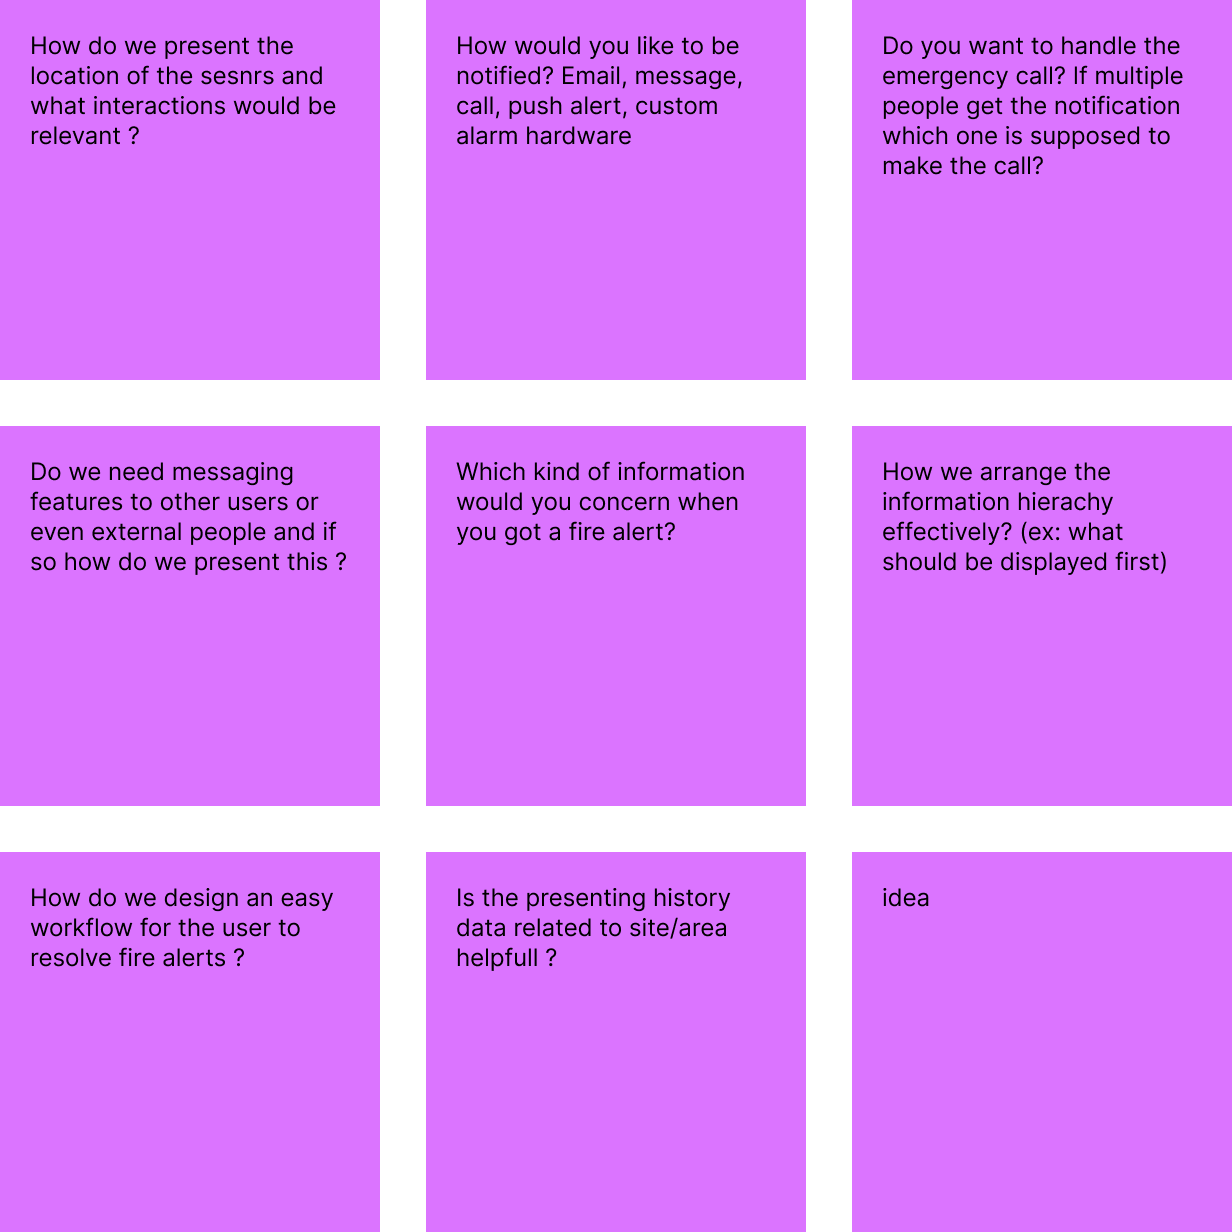
\includegraphics[width=10cm]{lotus_blossom_bottom_right}
  \caption{Ergebnis lotus blossom unten rechts}
  \label{fig:lotus_blossom_bottom_right}
\end{figure}
\begin{figure}[H]
  \centering
  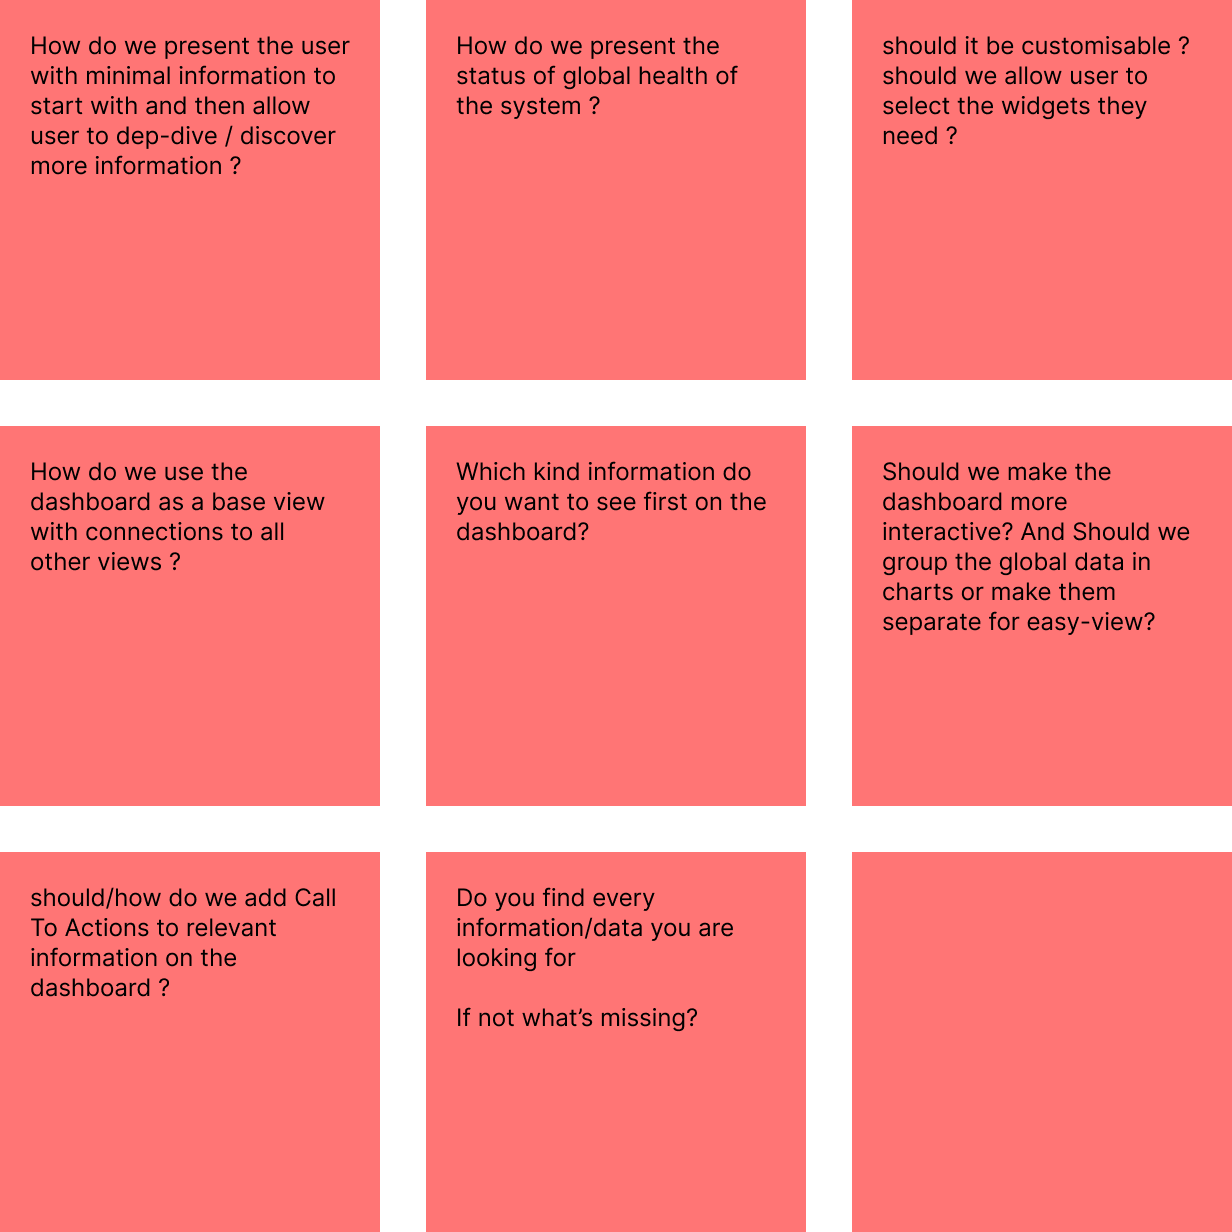
\includegraphics[width=10cm]{lotus_blossom_bottom}
  \caption{Ergebnis lotus blossom unten}
  \label{fig:lotus_blossom_bottom}
\end{figure}
\begin{figure}[H]
  \centering
  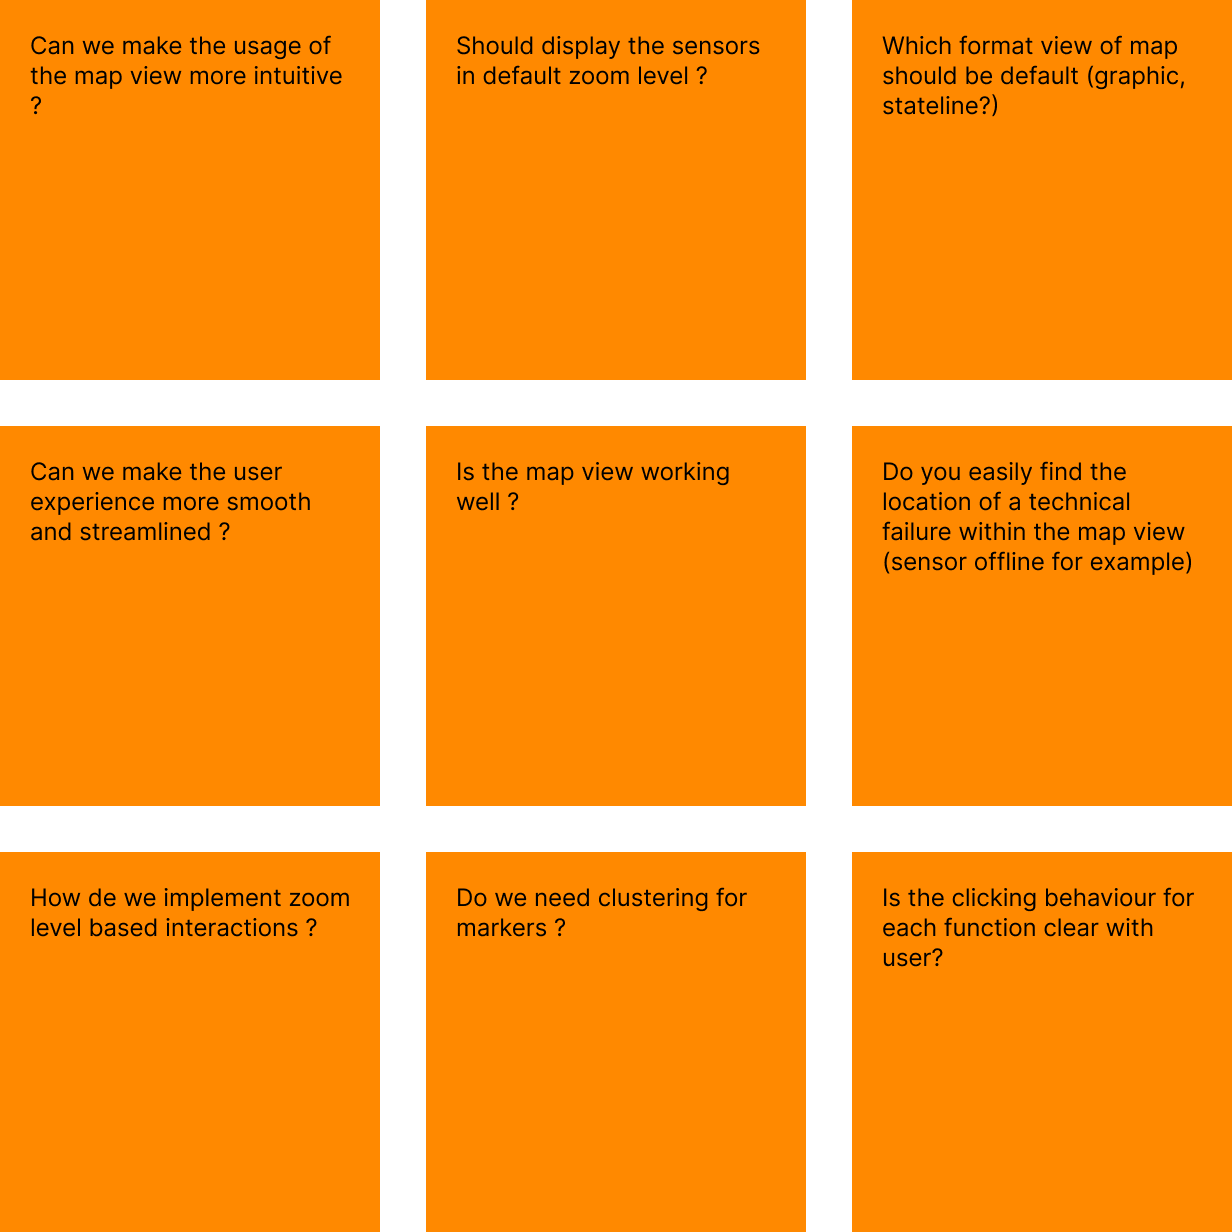
\includegraphics[width=10cm]{lotus_blossom_bottom_left}
  \caption{Ergebnis lotus blossom unten links}
  \label{fig:lotus_blossom_bottom_left}
\end{figure}
\begin{figure}[H]
  \centering
  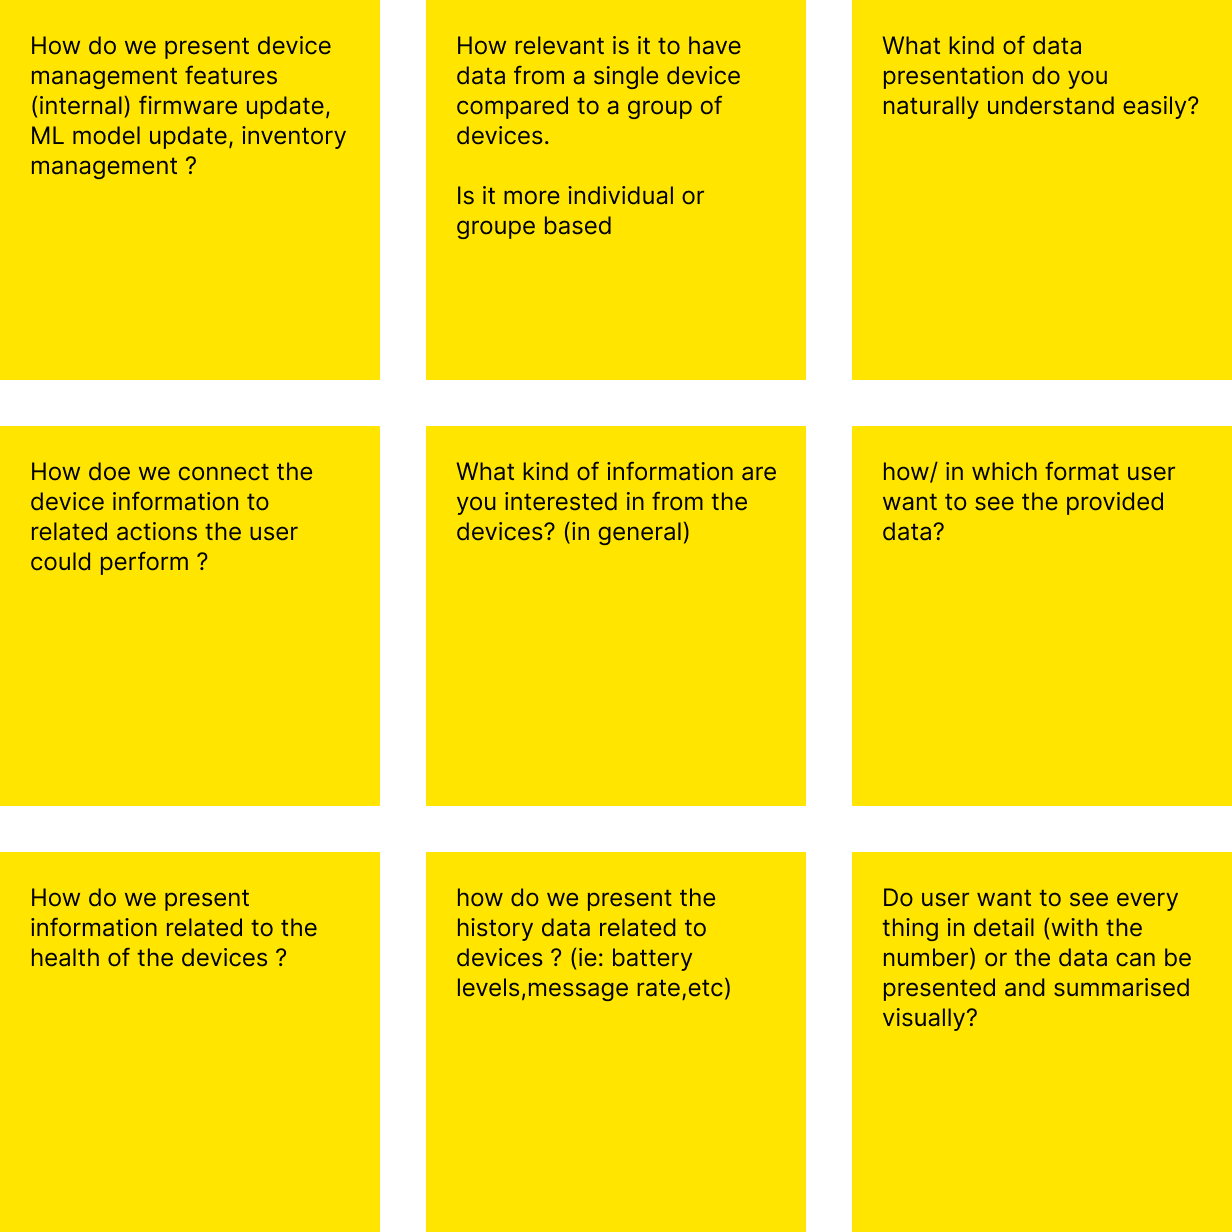
\includegraphics[width=10cm]{lotus_blossom_top_left}
  \caption{Ergebnis lotus blossom oben links}
  \label{fig:lotus_blossom_top_left}
\end{figure}